% Options for packages loaded elsewhere
\PassOptionsToPackage{unicode}{hyperref}
\PassOptionsToPackage{hyphens}{url}
%
\documentclass[
]{article}
\title{SLR}
\author{Brooke Wheeler}
\date{1/26/2022}

\usepackage{amsmath,amssymb}
\usepackage{lmodern}
\usepackage{iftex}
\ifPDFTeX
  \usepackage[T1]{fontenc}
  \usepackage[utf8]{inputenc}
  \usepackage{textcomp} % provide euro and other symbols
\else % if luatex or xetex
  \usepackage{unicode-math}
  \defaultfontfeatures{Scale=MatchLowercase}
  \defaultfontfeatures[\rmfamily]{Ligatures=TeX,Scale=1}
\fi
% Use upquote if available, for straight quotes in verbatim environments
\IfFileExists{upquote.sty}{\usepackage{upquote}}{}
\IfFileExists{microtype.sty}{% use microtype if available
  \usepackage[]{microtype}
  \UseMicrotypeSet[protrusion]{basicmath} % disable protrusion for tt fonts
}{}
\makeatletter
\@ifundefined{KOMAClassName}{% if non-KOMA class
  \IfFileExists{parskip.sty}{%
    \usepackage{parskip}
  }{% else
    \setlength{\parindent}{0pt}
    \setlength{\parskip}{6pt plus 2pt minus 1pt}}
}{% if KOMA class
  \KOMAoptions{parskip=half}}
\makeatother
\usepackage{xcolor}
\IfFileExists{xurl.sty}{\usepackage{xurl}}{} % add URL line breaks if available
\IfFileExists{bookmark.sty}{\usepackage{bookmark}}{\usepackage{hyperref}}
\hypersetup{
  pdftitle={SLR},
  pdfauthor={Brooke Wheeler},
  hidelinks,
  pdfcreator={LaTeX via pandoc}}
\urlstyle{same} % disable monospaced font for URLs
\usepackage[margin=1in]{geometry}
\usepackage{color}
\usepackage{fancyvrb}
\newcommand{\VerbBar}{|}
\newcommand{\VERB}{\Verb[commandchars=\\\{\}]}
\DefineVerbatimEnvironment{Highlighting}{Verbatim}{commandchars=\\\{\}}
% Add ',fontsize=\small' for more characters per line
\usepackage{framed}
\definecolor{shadecolor}{RGB}{248,248,248}
\newenvironment{Shaded}{\begin{snugshade}}{\end{snugshade}}
\newcommand{\AlertTok}[1]{\textcolor[rgb]{0.94,0.16,0.16}{#1}}
\newcommand{\AnnotationTok}[1]{\textcolor[rgb]{0.56,0.35,0.01}{\textbf{\textit{#1}}}}
\newcommand{\AttributeTok}[1]{\textcolor[rgb]{0.77,0.63,0.00}{#1}}
\newcommand{\BaseNTok}[1]{\textcolor[rgb]{0.00,0.00,0.81}{#1}}
\newcommand{\BuiltInTok}[1]{#1}
\newcommand{\CharTok}[1]{\textcolor[rgb]{0.31,0.60,0.02}{#1}}
\newcommand{\CommentTok}[1]{\textcolor[rgb]{0.56,0.35,0.01}{\textit{#1}}}
\newcommand{\CommentVarTok}[1]{\textcolor[rgb]{0.56,0.35,0.01}{\textbf{\textit{#1}}}}
\newcommand{\ConstantTok}[1]{\textcolor[rgb]{0.00,0.00,0.00}{#1}}
\newcommand{\ControlFlowTok}[1]{\textcolor[rgb]{0.13,0.29,0.53}{\textbf{#1}}}
\newcommand{\DataTypeTok}[1]{\textcolor[rgb]{0.13,0.29,0.53}{#1}}
\newcommand{\DecValTok}[1]{\textcolor[rgb]{0.00,0.00,0.81}{#1}}
\newcommand{\DocumentationTok}[1]{\textcolor[rgb]{0.56,0.35,0.01}{\textbf{\textit{#1}}}}
\newcommand{\ErrorTok}[1]{\textcolor[rgb]{0.64,0.00,0.00}{\textbf{#1}}}
\newcommand{\ExtensionTok}[1]{#1}
\newcommand{\FloatTok}[1]{\textcolor[rgb]{0.00,0.00,0.81}{#1}}
\newcommand{\FunctionTok}[1]{\textcolor[rgb]{0.00,0.00,0.00}{#1}}
\newcommand{\ImportTok}[1]{#1}
\newcommand{\InformationTok}[1]{\textcolor[rgb]{0.56,0.35,0.01}{\textbf{\textit{#1}}}}
\newcommand{\KeywordTok}[1]{\textcolor[rgb]{0.13,0.29,0.53}{\textbf{#1}}}
\newcommand{\NormalTok}[1]{#1}
\newcommand{\OperatorTok}[1]{\textcolor[rgb]{0.81,0.36,0.00}{\textbf{#1}}}
\newcommand{\OtherTok}[1]{\textcolor[rgb]{0.56,0.35,0.01}{#1}}
\newcommand{\PreprocessorTok}[1]{\textcolor[rgb]{0.56,0.35,0.01}{\textit{#1}}}
\newcommand{\RegionMarkerTok}[1]{#1}
\newcommand{\SpecialCharTok}[1]{\textcolor[rgb]{0.00,0.00,0.00}{#1}}
\newcommand{\SpecialStringTok}[1]{\textcolor[rgb]{0.31,0.60,0.02}{#1}}
\newcommand{\StringTok}[1]{\textcolor[rgb]{0.31,0.60,0.02}{#1}}
\newcommand{\VariableTok}[1]{\textcolor[rgb]{0.00,0.00,0.00}{#1}}
\newcommand{\VerbatimStringTok}[1]{\textcolor[rgb]{0.31,0.60,0.02}{#1}}
\newcommand{\WarningTok}[1]{\textcolor[rgb]{0.56,0.35,0.01}{\textbf{\textit{#1}}}}
\usepackage{graphicx}
\makeatletter
\def\maxwidth{\ifdim\Gin@nat@width>\linewidth\linewidth\else\Gin@nat@width\fi}
\def\maxheight{\ifdim\Gin@nat@height>\textheight\textheight\else\Gin@nat@height\fi}
\makeatother
% Scale images if necessary, so that they will not overflow the page
% margins by default, and it is still possible to overwrite the defaults
% using explicit options in \includegraphics[width, height, ...]{}
\setkeys{Gin}{width=\maxwidth,height=\maxheight,keepaspectratio}
% Set default figure placement to htbp
\makeatletter
\def\fps@figure{htbp}
\makeatother
\setlength{\emergencystretch}{3em} % prevent overfull lines
\providecommand{\tightlist}{%
  \setlength{\itemsep}{0pt}\setlength{\parskip}{0pt}}
\setcounter{secnumdepth}{-\maxdimen} % remove section numbering
\ifLuaTeX
  \usepackage{selnolig}  % disable illegal ligatures
\fi

\begin{document}
\maketitle

\begin{Shaded}
\begin{Highlighting}[]
\FunctionTok{library}\NormalTok{(tidyverse)}
\end{Highlighting}
\end{Shaded}

\begin{verbatim}
## -- Attaching packages --------------------------------------- tidyverse 1.3.1 --
\end{verbatim}

\begin{verbatim}
## v ggplot2 3.3.5     v purrr   0.3.4
## v tibble  3.1.6     v dplyr   1.0.7
## v tidyr   1.1.4     v stringr 1.4.0
## v readr   2.1.1     v forcats 0.5.1
\end{verbatim}

\begin{verbatim}
## -- Conflicts ------------------------------------------ tidyverse_conflicts() --
## x dplyr::filter() masks stats::filter()
## x dplyr::lag()    masks stats::lag()
\end{verbatim}

\begin{Shaded}
\begin{Highlighting}[]
\FunctionTok{getwd}\NormalTok{()}
\end{Highlighting}
\end{Shaded}

\begin{verbatim}
## [1] "/Users/brookewheeler/Desktop/Regression/Labs"
\end{verbatim}

\begin{Shaded}
\begin{Highlighting}[]
\NormalTok{House }\OtherTok{\textless{}{-}} \FunctionTok{read.csv}\NormalTok{(}\StringTok{"../Data/HOME\_SAlES.csv"}\NormalTok{)}
\FunctionTok{attach}\NormalTok{(House)}
\end{Highlighting}
\end{Shaded}

\hypertarget{find-correlation-and-covariance-between-house-prices-and-house-sizes.-what-do-these-values-indicate}{%
\section{1. Find correlation and covariance between house prices and
house sizes. What do these values
indicate?}\label{find-correlation-and-covariance-between-house-prices-and-house-sizes.-what-do-these-values-indicate}}

\begin{Shaded}
\begin{Highlighting}[]
\FunctionTok{cor}\NormalTok{(SALES\_PRICE, FINISHED\_AREA)}
\end{Highlighting}
\end{Shaded}

\begin{verbatim}
## [1] 0.8194701
\end{verbatim}

\begin{Shaded}
\begin{Highlighting}[]
\FunctionTok{cov}\NormalTok{(SALES\_PRICE, FINISHED\_AREA)}
\end{Highlighting}
\end{Shaded}

\begin{verbatim}
## [1] 80367.58
\end{verbatim}

\begin{Shaded}
\begin{Highlighting}[]
\CommentTok{\# The correlation value is closer to 1 than 0 meaning that linear relationship between sales price and house size is strong. The covariance value is positive, showing that as sales price increases so does house size and as house size increases so does sales price. }
\end{Highlighting}
\end{Shaded}

\hypertarget{scatterplot}{%
\section{2. Scatterplot}\label{scatterplot}}

\begin{Shaded}
\begin{Highlighting}[]
\FunctionTok{plot}\NormalTok{(FINISHED\_AREA, SALES\_PRICE)}
\end{Highlighting}
\end{Shaded}

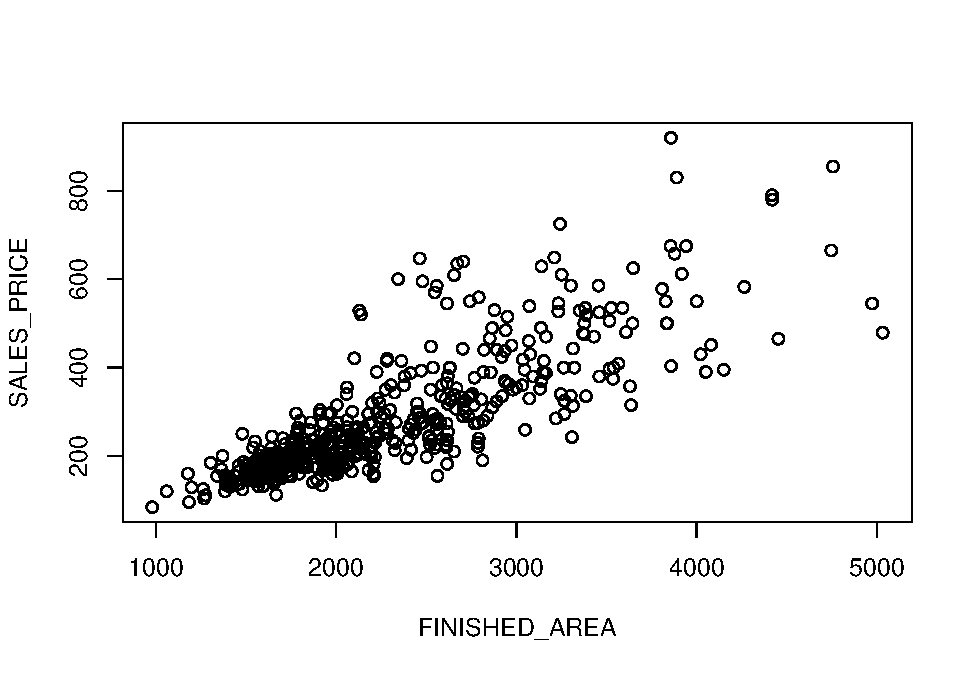
\includegraphics{SLR_files/figure-latex/unnamed-chunk-3-1.pdf}

\hypertarget{find-equation-of-least-squares-regression-line.-find-regression-coefficients.}{%
\section{3. Find equation of least-squares regression line. Find
regression
coefficients.}\label{find-equation-of-least-squares-regression-line.-find-regression-coefficients.}}

\begin{Shaded}
\begin{Highlighting}[]
\CommentTok{\#y first}
\NormalTok{reg }\OtherTok{\textless{}{-}} \FunctionTok{lm}\NormalTok{(SALES\_PRICE }\SpecialCharTok{\textasciitilde{}}\NormalTok{ FINISHED\_AREA, }\AttributeTok{data =}\NormalTok{ House)}
\NormalTok{reg}
\end{Highlighting}
\end{Shaded}

\begin{verbatim}
## 
## Call:
## lm(formula = SALES_PRICE ~ FINISHED_AREA, data = House)
## 
## Coefficients:
##   (Intercept)  FINISHED_AREA  
##       -81.433          0.159
\end{verbatim}

\begin{Shaded}
\begin{Highlighting}[]
\CommentTok{\# y (hat)= {-}81.433 + .159}
\end{Highlighting}
\end{Shaded}

\hypertarget{plot-regression-line}{%
\section{4. Plot regression line}\label{plot-regression-line}}

\begin{Shaded}
\begin{Highlighting}[]
\NormalTok{reg}
\end{Highlighting}
\end{Shaded}

\begin{verbatim}
## 
## Call:
## lm(formula = SALES_PRICE ~ FINISHED_AREA, data = House)
## 
## Coefficients:
##   (Intercept)  FINISHED_AREA  
##       -81.433          0.159
\end{verbatim}

\begin{Shaded}
\begin{Highlighting}[]
\FunctionTok{plot}\NormalTok{(FINISHED\_AREA, SALES\_PRICE)}
\FunctionTok{abline}\NormalTok{(reg, }\AttributeTok{col =} \StringTok{"blue"}\NormalTok{)}
\end{Highlighting}
\end{Shaded}

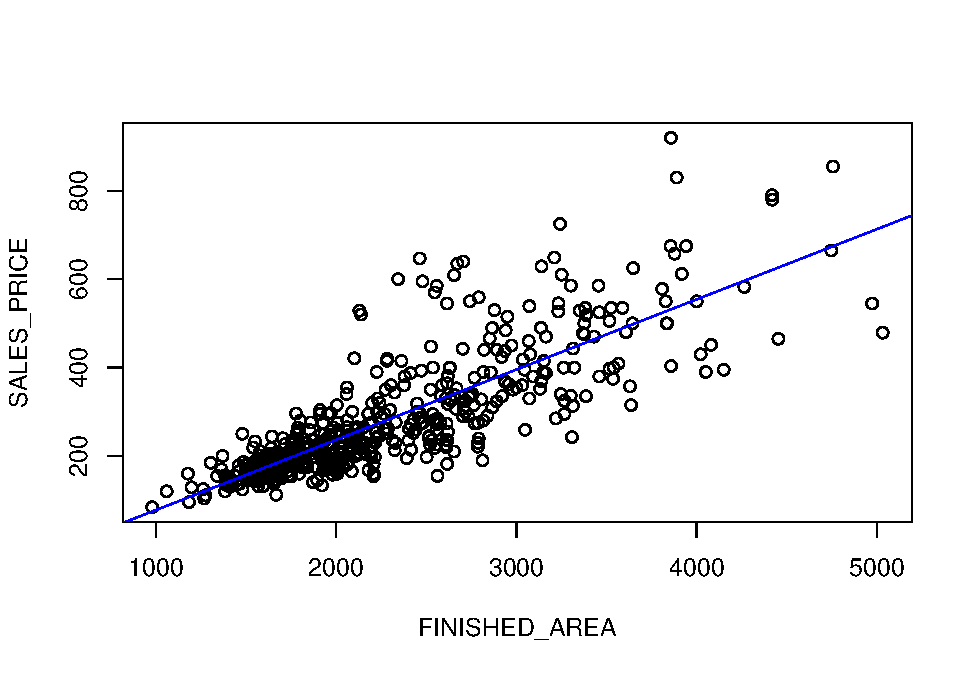
\includegraphics{SLR_files/figure-latex/unnamed-chunk-5-1.pdf}

\hypertarget{create-a-new-plot-that-shows-all-predicted-house-prices-using-new-color-for-points}{%
\subsection{5. Create a new plot that shows all predicted house prices,
using new color for
points}\label{create-a-new-plot-that-shows-all-predicted-house-prices-using-new-color-for-points}}

\begin{Shaded}
\begin{Highlighting}[]
\NormalTok{reg}
\end{Highlighting}
\end{Shaded}

\begin{verbatim}
## 
## Call:
## lm(formula = SALES_PRICE ~ FINISHED_AREA, data = House)
## 
## Coefficients:
##   (Intercept)  FINISHED_AREA  
##       -81.433          0.159
\end{verbatim}

\begin{Shaded}
\begin{Highlighting}[]
\FunctionTok{plot}\NormalTok{(FINISHED\_AREA, SALES\_PRICE)}
\FunctionTok{abline}\NormalTok{(reg, }\AttributeTok{col =} \StringTok{"blue"}\NormalTok{)}

\NormalTok{Yhat }\OtherTok{\textless{}{-}} \FunctionTok{predict}\NormalTok{(reg, }\AttributeTok{x=}\NormalTok{ FINISHED\_AREA)}

\FunctionTok{points}\NormalTok{(FINISHED\_AREA, Yhat, }\AttributeTok{col=}\StringTok{"blue"}\NormalTok{)}
\end{Highlighting}
\end{Shaded}

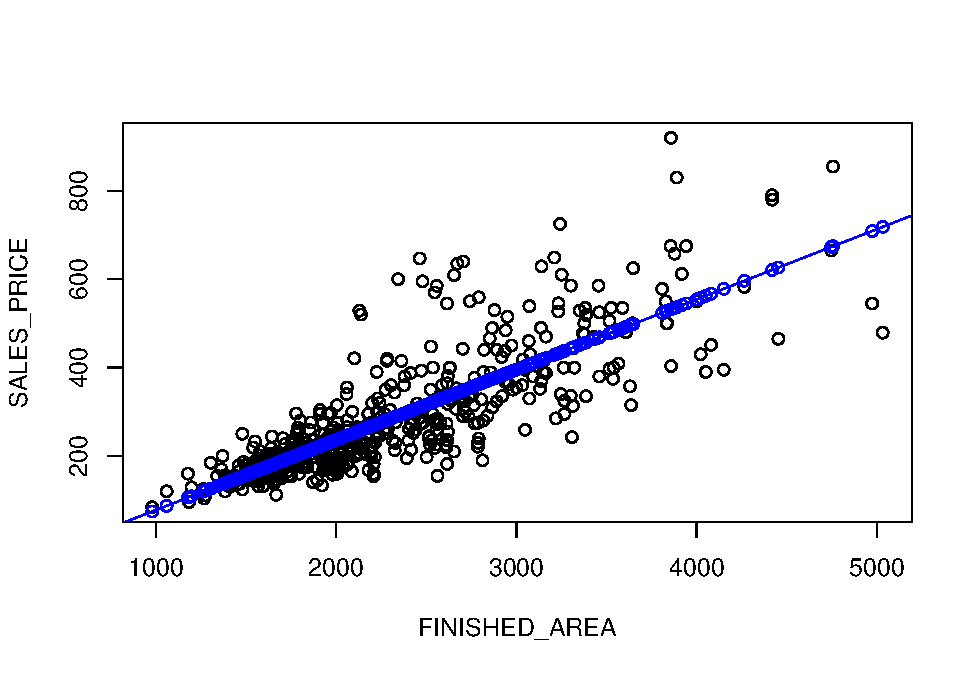
\includegraphics{SLR_files/figure-latex/unnamed-chunk-6-1.pdf}

\hypertarget{if-the-size-of-a-house-is-2000-square-feet-what-is-the-predicted-house-price-also-show-predictions-for-houses-that-are-1500-and-3500-square-feet.}{%
\subsection{6. If the size of a house is 2000 square feet, what is the
predicted house price? Also, show predictions for houses that are 1500
and 3500 square
feet.}\label{if-the-size-of-a-house-is-2000-square-feet-what-is-the-predicted-house-price-also-show-predictions-for-houses-that-are-1500-and-3500-square-feet.}}

\begin{Shaded}
\begin{Highlighting}[]
\FunctionTok{predict}\NormalTok{(reg, }\FunctionTok{data.frame}\NormalTok{(}\AttributeTok{FINISHED\_AREA =} \DecValTok{2000}\NormalTok{))}
\end{Highlighting}
\end{Shaded}

\begin{verbatim}
##        1 
## 236.4675
\end{verbatim}

\begin{Shaded}
\begin{Highlighting}[]
\CommentTok{\# predicted house price for 2000 square feet is 236.4675 thousand $}

\FunctionTok{predict}\NormalTok{(reg, }\FunctionTok{data.frame}\NormalTok{(}\AttributeTok{FINISHED\_AREA =} \DecValTok{1500}\NormalTok{))}
\end{Highlighting}
\end{Shaded}

\begin{verbatim}
##        1 
## 156.9924
\end{verbatim}

\begin{Shaded}
\begin{Highlighting}[]
\FunctionTok{predict}\NormalTok{(reg, }\FunctionTok{data.frame}\NormalTok{(}\AttributeTok{FINISHED\_AREA =} \DecValTok{3500}\NormalTok{))}
\end{Highlighting}
\end{Shaded}

\begin{verbatim}
##        1 
## 474.8929
\end{verbatim}

\hypertarget{find-values-of-all-residuals}{%
\subsection{7. Find values of all
residuals}\label{find-values-of-all-residuals}}

\begin{Shaded}
\begin{Highlighting}[]
\FunctionTok{resid}\NormalTok{(reg)}
\end{Highlighting}
\end{Shaded}

\begin{verbatim}
##             1             2             3             4             5 
##  -40.50415343   94.31337139   48.50153555   26.57246833    7.87823953 
##             6             7             8             9            10 
##   16.93679262  -40.90076508  -22.41057221   18.61567202  -72.65270969 
##            11            12            13            14            15 
## -175.53510265  196.80285220   79.02221602   56.62409802   49.12696400 
##            16            17            18            19            20 
##   94.70580041   12.58969972  -19.95333764  -54.03322065   -8.65122484 
##            21            22            23            24            25 
##   41.60948217   13.20368947  -73.64478456  -75.72188568 -142.69850743 
##            26            27            28            29            30 
##  -68.74651984  -33.53535308  -30.68353369 -109.52916324 -144.04735712 
##            31            32            33            34            35 
##   13.86560941  -42.30063987 -115.52916324  -53.47964448  -66.16347931 
##            36            37            38            39            40 
##  -75.78851061 -201.87441713 -152.38085741   27.36560941    2.19158171 
##            41            42            43            44            45 
##   14.86560941   20.14959095   -4.18997397   -1.70222844  -20.20841829 
##            46            47            48            49            50 
##  -30.35647368  -39.02780360  -74.93669122  -64.50762400    9.18041495 
##            51            52            53            54            55 
##  -28.19294368    3.64340110  -71.69603860    9.66172020 -170.79754494 
##            56            57            58            59            60 
##   75.21161461  -16.11594627  138.54956945  108.99547092  -85.29618531 
##            61            62            63            64            65 
##   -5.34248392   -8.24664506  -18.75446647  -53.95204062   -0.54476306 
##            66            67            68            69            70 
##  -23.91582106   -7.71205706  -57.08326177  259.83825598   -4.46797685 
##            71            72            73            74            75 
##  129.85113654  293.27549877  388.36190616  180.46564866  142.07928426 
##            76            77            78            79            80 
##   62.55278959  169.19082667   -7.94484904  291.11629810  336.77957768 
##            81            82            83            84            85 
##  159.03187644  122.68290154   54.15046747   44.81696718   98.64926781 
##            86            87            88            89            90 
##  268.57903382  291.71792967   62.22746487  126.68250440  117.70389894 
##            91            92            93            94            95 
##  -46.54077013   23.57014620  220.20270549   46.11951824  291.47257205 
##            96            97            98            99           100 
##  308.85360537  -13.83083778  210.77809282  -12.05948637  282.39532421 
##           101           102           103           104           105 
##  174.68574603  246.58670852 -239.40461505 -164.02655143    6.02345044 
##           106           107           108           109           110 
##  211.48817188   28.06393486  271.77790500  -15.24493127   77.79072295 
##           111           112           113           114           115 
##   72.96502257   56.13338278   70.82489231   94.44942274    2.21830532 
##           116           117           118           119           120 
##  132.13783734  113.04685018   41.61617289 -112.69850743  -18.88073219 
##           121           122           123           124           125 
##    6.23365471   81.50797583  153.97418212   78.17621083 -128.29704408 
##           126           127           128           129           130 
##  195.59141351  -88.53485221  -28.30013900 -161.37243141 -115.58399532 
##           131           132           133           134           135 
## -107.26176551   22.97146285   58.87391019   73.03434528  127.52976550 
##           136           137           138           139           140 
##  120.99250122  -30.04116727  115.38158489   23.92961879   53.77363827 
##           141           142           143           144           145 
##   83.03139706  117.76868284   -2.57991641  143.67980662   61.74887889 
##           146           147           148           149           150 
##  -27.66433807   48.51441611  -17.51665833   22.50203642 -127.86488193 
##           151           152           153           154           155 
##   19.65801694   16.15318674  -81.25087068   -7.57050643 -183.21051147 
##           156           157           158           159           160 
##   94.81943601   85.54498968   10.35373059   69.98012153   52.38706873 
##           161           162           163           164           165 
##  127.42466337   10.66383114  -64.24022628  -26.66483894 -131.82811851 
##           166           167           168           169           170 
##   56.97393169   63.23488913  -12.87776249  -16.63388972  -37.16270651 
##           171           172           173           174           175 
##   23.60529954  -29.94238020   30.11914259 -138.05639145   65.84419539 
##           176           177           178           179           180 
##   49.79480185  -65.84384356  133.70851968   -2.32811851   12.37353454 
##           181           182           183           184           185 
##   -2.95030533  -78.98570911   16.86004565   45.38442938   61.22993370 
##           186           187           188           189           190 
##   45.98334167   96.18660479   30.06974906  -47.85287789  -24.18462140 
##           191           192           193           194           195 
##  -76.38357668  -13.46107495  -26.74183635  -33.98558389   -6.68662861 
##           196           197           198           199           200 
##  -50.53483072  -47.70172757  -49.52594310  -36.42245103  -20.45488510 
##           201           202           203           204           205 
##  -80.43606514 -105.81506975  261.59735292  -25.59378095   30.23934369 
##           206           207           208           209           210 
##   -4.57818112 -108.68610625   18.99547092   -7.77721863 -172.31548839 
##           211           212           213           214           215 
##  -31.27291078  -76.86216266   30.08361360  -64.11841511  -94.51950282 
##           216           217           218           219           220 
##  -41.84532841   19.84741553   61.68551709 -181.51009284   72.83800555 
##           221           222           223           224           225 
##  -29.96357985 -121.77253513   55.53260999   65.30099170   34.67757046 
##           226           227           228           229           230 
##  -99.53980764  -96.74505648  -36.59202417    5.83060278   46.05711893 
##           231           232           233           234           235 
##  -29.45662039  -39.27613092  168.47851146   51.74243861   23.98309124 
##           236           237           238           239           240 
##   37.41983316 -111.74505648   -6.27734385  -60.24505648 -105.07224171 
##           241           242           243           244           245 
##   18.61765774  -20.44127100  -36.57370507  -10.83462140  -42.90549157 
##           246           247           248           249           250 
##   77.89668385   94.00688812  -12.22673739  -12.92109140  -93.12163525 
##           251           252           253           254           255 
##  -85.39323710    5.76397785  -87.52916324   23.00760018    0.13436677 
##           256           257           258           259           260 
##  -46.72351725 -113.84505648   15.93382291  -63.13698464   27.29183215 
##           261           262           263           264           265 
##  -40.51774604  -39.68340848  -36.53547830   -8.57518992  -86.82029711 
##           266           267           268           269           270 
##  -88.59081125  -21.81611448    7.55578079   21.21916409   22.26876694 
##           271           272           273           274           275 
##  -65.04760755  -34.40883692  -40.63859471   20.45214201   15.17744525 
##           276           277           278           279           280 
##  -63.93613092  -52.49821401  -13.77303600   -2.85647368 -145.22784659 
##           281           282           283           284           285 
## -130.42096618   75.00463047    7.88578901 -140.40239665   53.27623232 
##           286           287           288           289           290 
##  -84.54129249  -20.24518170  -36.51812169  -80.11665833   64.11876694 
##           291           292           293           294           295 
##   -5.66508938  -14.90574200  -51.21893747   -2.49227460    9.75159816 
##           296           297           298           299           300 
##    8.28564230  -53.34074864  -23.78972354   17.44582695   11.18982493 
##           301           302           303           304           305 
##  -14.26239160  -12.91515199  -18.16199445  -35.01046849   10.09425800 
##           306           307           308           309           310 
##  -31.33602215  -53.93050138    4.03235956  -33.04154292    4.37204969 
##           311           312           313           314           315 
##   30.74568847   31.83633287   23.54043140   15.83033085  -12.70829307 
##           316           317           318           319           320 
##   35.25644986   14.13733647 -110.31820579  -32.49026739   10.10638725 
##           321           322           323           324           325 
##   29.04473924   27.87987110   19.62508200   -8.92303600  -68.48595954 
##           326           327           328           329           330 
##  -29.70816785  -21.65122484  -24.44894569  -56.89955216  -27.33480923 
##           331           332           333           334           335 
##    0.85335494  -52.54894569   32.09722770  -11.04166814  -19.06617709 
##           336           337           338           339           340 
##   -3.80250037    1.08175309  -29.03844800   50.42280286   37.95214201 
##           341           342           343           344           345 
##  -49.52594310   24.16506556  -86.17090357  -33.59254653  -16.68353369 
##           346           347           348           349           350 
##    5.86585984  -37.76362602  -12.19415660  -58.20952749   38.70456786 
##           351           352           353           354           355 
##  -47.62176047   -3.94139621   11.79492707 -118.76053109  -18.66236029 
##           356           357           358           359           360 
##  -44.01071892    7.19170693   13.59716509  -48.14342492  -29.48756961 
##           361           362           363           364           365 
## -122.64714780  -76.16793386  -11.09415660  -50.34099907   -0.25781182 
##           366           367           368           369           370 
##   17.51688494  -10.66098883   -1.75277230   10.47623232   -4.85189391 
##           371           372           373           374           375 
##   -5.08177691  -25.92431153   -6.06320738  -13.85498883  -41.44894569 
##           376           377           378           379           380 
##  -57.58016684  -61.54530692  -75.12634024  -57.62176047  -61.16347931 
##           381           382           383           384           385 
##  -29.22807553  -33.47370507    6.95711893  -43.98271791    0.29158171 
##           386           387           388           389           390 
##  -20.15404783    0.71755402   -0.45835568   -3.98298984   12.10019741 
##           391           392           393           394           395 
##  -31.13547830   32.94570174   11.64959095   67.96008864 -131.66134688 
##           396           397           398           399           400 
##   13.45699372  -56.12309861  -59.26214116    9.06949862  -49.08784154 
##           401           402           403           404           405 
##    7.48148117   -9.85028384   23.13263148   -1.15283491   12.38417894 
##           406           407           408           409           410 
##  -15.27140444   51.59413278  -14.27019151  -11.10034645   30.92144323 
##           411           412           413           414           415 
##   31.73290341   34.62483157   55.64959095   13.84097525   11.55396140 
##           416           417           418           419           420 
##  -52.56630230   -2.87033822  -73.14181485   26.78430416   21.73599833 
##           421           422           423           424           425 
##  -31.20802114  -39.89160553  -17.61582106  -28.60963121  -14.77746907 
##           426           427           428           429           430 
##  -15.88742290   17.06008864   18.25948217   -4.88123306   24.00638725 
##           431           432           433           434           435 
##   -9.33183952  -20.93493444   -0.06764044  -55.20950600  -37.67598421 
##           436           437           438           439           440 
##  -28.33305245    2.83788033   -9.81582106  -11.21770305  -51.83790415 
##           441           442           443           444           445 
##  -15.03991136    6.01379002  -25.48311506    6.06506556   13.07422511 
##           446           447           448           449           450 
##  -42.39769165  -13.00477951  -97.17855677   -4.51824691    5.11257710 
##           451           452           453           454           455 
##  -10.38754812   23.62186186   -8.31945983   19.60032263  -13.60963121 
##           456           457           458           459           460 
##   13.58794294  -98.84384356   -8.84085236   -5.80720536   11.88457609 
##           461           462           463           464           465 
##  -40.25162198 -103.77600571  -40.51205706  -18.65417305   -2.33802937 
##           466           467           468           469           470 
##   81.67905531   13.29777156   -0.37370507  -50.87491800    1.70207941 
##           471           472           473           474           475 
##  -16.71609298  -28.22067276  -13.88432798   -1.52322383  -18.41582106 
##           476           477           478           479           480 
##   -4.06939722  -45.30089030   22.66197063  -18.88123306  -14.04488828 
##           481           482           483           484           485 
##   18.38417894  -27.67073537    5.71002603  -19.01393906  -42.99685438 
##           486           487           488           489           490 
##  -70.73911707    8.76506556    0.60948217   13.75147294  -26.06333260 
##           491           492           493           494           495 
##  -77.83911707  -15.52322383  -67.03077331  -15.39670767  -21.70222844 
##           496           497           498           499           500 
##  -38.78244598  -12.65592983  -14.12510582  -38.08183952    6.51997987 
##           501           502           503           504           505 
##  -43.39785799   14.85026002  -47.28851061   -0.56157582   54.18957450 
##           506           507           508           509           510 
##    5.67880488   63.50824776   58.66184542   23.43963711  -16.37046344 
##           511           512           513           514           515 
##    2.99522049   20.01056988    0.08781772   63.67113018  -20.44421921 
##           516           517           518           519           520 
##  -35.64206529   -5.62792882  -44.62968560  -42.56630230  -90.56939722 
##           521           522 
##  -29.81339521  -11.26412689
\end{verbatim}

\hypertarget{look-at-the-first-house.-calc.-the-residual-value}{%
\subsection{8. Look at the first house. Calc. the residual
value}\label{look-at-the-first-house.-calc.-the-residual-value}}

\begin{Shaded}
\begin{Highlighting}[]
\FunctionTok{predict}\NormalTok{(reg, }\FunctionTok{data.frame}\NormalTok{(}\AttributeTok{FINISHED\_AREA =} \DecValTok{3032}\NormalTok{))}
\end{Highlighting}
\end{Shaded}

\begin{verbatim}
##        1 
## 400.5042
\end{verbatim}

\hypertarget{one-property-we-discussed-is-that-the-sum-of-the-residuals-is-zero.-find-the-sum-of-the-residuals-here-and-comment-on-the-value-that-you-obtain.}{%
\subsection{9. One property we discussed is that the sum of the
residuals is zero. Find the sum of the residuals here and comment on the
value that you
obtain.}\label{one-property-we-discussed-is-that-the-sum-of-the-residuals-is-zero.-find-the-sum-of-the-residuals-here-and-comment-on-the-value-that-you-obtain.}}

\begin{Shaded}
\begin{Highlighting}[]
\FunctionTok{sum}\NormalTok{(}\FunctionTok{resid}\NormalTok{(reg))}
\end{Highlighting}
\end{Shaded}

\begin{verbatim}
## [1] -2.375877e-13
\end{verbatim}

\begin{Shaded}
\begin{Highlighting}[]
\CommentTok{\#The value I obtained is very very close to one which would make sense if the expected value is zero. }
\end{Highlighting}
\end{Shaded}

\hypertarget{show-the-regression-line-passes-through-x-y-.-hint-first-find-the-means-and-then-predict-the-appropriate-value.}{%
\subsection{10. Show the regression line passes through (X ̅,Y ̅). Hint:
First find the means and then predict the appropriate
value.}\label{show-the-regression-line-passes-through-x-y-.-hint-first-find-the-means-and-then-predict-the-appropriate-value.}}

\begin{Shaded}
\begin{Highlighting}[]
\FunctionTok{summary}\NormalTok{(House)}
\end{Highlighting}
\end{Shaded}

\begin{verbatim}
##        ID         SALES_PRICE    FINISHED_AREA     BEDROOMS       BATHROOMS    
##  Min.   :  1.0   Min.   : 84.0   Min.   : 980   Min.   :0.000   Min.   :0.000  
##  1st Qu.:131.2   1st Qu.:180.0   1st Qu.:1701   1st Qu.:3.000   1st Qu.:2.000  
##  Median :261.5   Median :229.9   Median :2061   Median :3.000   Median :3.000  
##  Mean   :261.5   Mean   :277.9   Mean   :2261   Mean   :3.471   Mean   :2.642  
##  3rd Qu.:391.8   3rd Qu.:335.0   3rd Qu.:2636   3rd Qu.:4.000   3rd Qu.:3.000  
##  Max.   :522.0   Max.   :920.0   Max.   :5032   Max.   :7.000   Max.   :7.000  
##   GARAGE_SIZE    YEAR_BUILT       STYLE          LOT_SIZE    
##  Min.   :0.0   Min.   :1885   Min.   :1.000   Min.   : 4560  
##  1st Qu.:2.0   1st Qu.:1956   1st Qu.:1.000   1st Qu.:17205  
##  Median :2.0   Median :1966   Median :2.000   Median :22200  
##  Mean   :2.1   Mean   :1967   Mean   :1.925   Mean   :24370  
##  3rd Qu.:2.0   3rd Qu.:1981   3rd Qu.:3.000   3rd Qu.:26787  
##  Max.   :7.0   Max.   :1998   Max.   :3.000   Max.   :86830  
##  AIR_CONDITIONER        POOL             QUALITY            HIGHWAY         
##  Length:522         Length:522         Length:522         Length:522        
##  Class :character   Class :character   Class :character   Class :character  
##  Mode  :character   Mode  :character   Mode  :character   Mode  :character  
##                                                                             
##                                                                             
## 
\end{verbatim}

\begin{Shaded}
\begin{Highlighting}[]
\CommentTok{\# mean sales price = 277.9}
\CommentTok{\# mean finished area = 2261}

\FunctionTok{predict}\NormalTok{(reg, }\FunctionTok{data.frame}\NormalTok{(}\AttributeTok{FINISHED\_AREA =} \DecValTok{2261}\NormalTok{))}
\end{Highlighting}
\end{Shaded}

\begin{verbatim}
##        1 
## 277.9535
\end{verbatim}

\begin{Shaded}
\begin{Highlighting}[]
\CommentTok{\# at x= 2261 y = 277.9535}
\end{Highlighting}
\end{Shaded}


\end{document}
